% Practice Test 07 — Alaska Edition
% Questions: 30 (18 MC + 12 SA)
% Generated by scripts/generate_practice_tests.py

\begin{practiceQuestion}{1-3-q23}{sa}
\begin{questionText}
Two quantities are proportional with $k = 7$. If $y = 56$, what is $x$?
\end{questionText}
\correctAnswer{$x = 8$}
\explanation{$y = kx$ so $56 = 7x$, giving $x = 56 \div 7 = 8$.}
\end{practiceQuestion}

\begin{practiceQuestion}{1-5-q09}{mc}
\begin{questionText}
The point $(1, r)$ on a proportional graph represents:
\end{questionText}
\choiceA{The total amount}
\choiceB{The unit rate}
\choiceC{The number of units}
\choiceD{The $y$-intercept}
\correctAnswer{B}
\explanation{At $x = 1$, $y = k \times 1 = k$. So the $y$-value at $x = 1$ is the unit rate.}
\end{practiceQuestion}

\begin{practiceQuestion}{1-6-q29}{gsa}
\begin{questionText}
The double number line below relates inches on a blueprint to actual feet. A hallway measures $3.5$ inches on the blueprint. What is the actual length?

\begin{center}
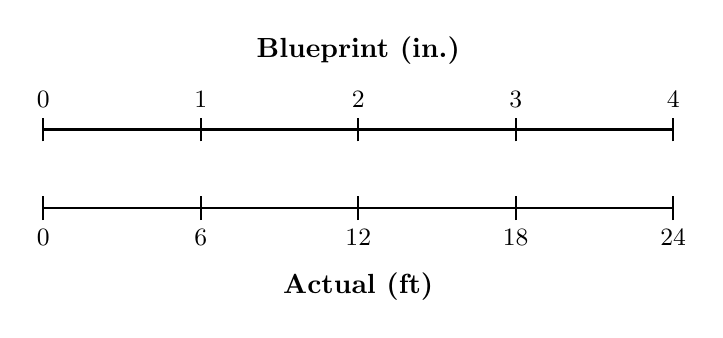
\begin{tikzpicture}[scale=1.0]
  % Top: blueprint inches
  \draw[thick] (0,1) -- (8,1);
  \foreach \x/\lab in {0/$0$, 2/$1$, 4/$2$, 6/$3$, 8/$4$} {
    \draw[thick] (\x,0.85) -- (\x,1.15);
    \node[above] at (\x,1.15) {\small \lab};
  }
  \node[above] at (4,1.7) {\textbf{Blueprint (in.)}};
  % Bottom: actual feet
  \draw[thick] (0,0) -- (8,0);
  \foreach \x/\lab in {0/$0$, 2/$6$, 4/$12$, 6/$18$, 8/$24$} {
    \draw[thick] (\x,-0.15) -- (\x,0.15);
    \node[below] at (\x,-0.15) {\small \lab};
  }
  \node[below] at (4,-0.7) {\textbf{Actual (ft)}};
\end{tikzpicture}
\end{center}
\end{questionText}
\correctAnswer{$21$ feet}
\explanation{Scale: $1$ inch $= 6$ feet. For $3.5$ inches: $6 \times 3.5 = 21$ feet.}
\end{practiceQuestion}

\begin{practiceQuestion}{2-2-q27}{gmc}
\begin{questionText}
The bar model below represents a whole amount. Use the model to find what percent the shaded part is of the whole.

\begin{center}
\begin{tikzpicture}[scale=0.65]
  % Whole bar divided into 8 equal parts, 3 shaded
  \foreach \i in {0,...,7} {
    \draw[thick] (\i*1,0) rectangle (\i*1+1,0.8);
  }
  \fill[funBlue!40] (0,0) rectangle (1,0.8);
  \fill[funBlue!40] (1,0) rectangle (2,0.8);
  \fill[funBlue!40] (2,0) rectangle (3,0.8);
  \foreach \i in {0,...,7} {
    \draw[thick] (\i*1,0) rectangle (\i*1+1,0.8);
  }
  \draw[thick,<->] (0,-0.4) -- (3,-0.4) node[midway,below,font=\small] {$45$};
  \draw[thick,<->] (0,-1.1) -- (8,-1.1) node[midway,below,font=\small] {Whole $= {?}$};
  \node[above,font=\small] at (1.5,0.8) {Shaded};
\end{tikzpicture}
\end{center}

If each section has the same value and there are $8$ equal sections total, what percent is shaded?
\end{questionText}
\choiceA{$25\%$}
\choiceB{$33\%$}
\choiceC{$37.5\%$}
\choiceD{$45\%$}
\correctAnswer{C}
\explanation{$3$ out of $8$ sections are shaded. $\frac{3}{8} = \frac{p}{100}$ → $p = 37.5\%$.}
\end{practiceQuestion}

\begin{practiceQuestion}{2-5-q19}{sa}
\begin{questionText}
A dinner bill is $\$64$. You leave an $18\%$ tip. How much is the tip?
\end{questionText}
\correctAnswer{$\$11.52$}
\explanation{$64 \times 0.18 = \$11.52$.}
\end{practiceQuestion}

\begin{practiceQuestion}{3-1-q21}{sa}
\begin{questionText}
Order from least to greatest: $-7, \; 3, \; -1, \; 0, \; -4$.
\end{questionText}
\correctAnswer{$-7, \; -4, \; -1, \; 0, \; 3$}
\explanation{On a number line from left to right: $-7 < -4 < -1 < 0 < 3$.}
\end{practiceQuestion}

\begin{practiceQuestion}{3-2-q12}{mc}
\begin{questionText}
What is $(-7) + 7 + (-3)$?
\end{questionText}
\choiceA{$-3$}
\choiceB{$3$}
\choiceC{$-17$}
\choiceD{$17$}
\correctAnswer{A}
\explanation{$(-7) + 7 = 0$ (opposites cancel). Then $0 + (-3) = -3$.}
\end{practiceQuestion}

\begin{practiceQuestion}{3-3-q04}{mc}
\begin{questionText}
What is $(-4) - (-4)$?
\end{questionText}
\choiceA{$-8$}
\choiceB{$8$}
\choiceC{$0$}
\choiceD{$-16$}
\correctAnswer{C}
\explanation{$(-4) - (-4) = (-4) + 4 = 0$. Any number minus itself equals $0$.}
\end{practiceQuestion}

\begin{practiceQuestion}{3-10-q16}{mc}
\begin{questionText}
The Dead Sea is at $-1{,}412$ feet elevation. A nearby cliff is $520$ feet above sea level. What is the distance between them?
\end{questionText}
\choiceA{$892$ ft}
\choiceB{$1{,}932$ ft}
\choiceC{$-892$ ft}
\choiceD{$-1{,}932$ ft}
\correctAnswer{B}
\explanation{$520 - (-1{,}412) = 520 + 1{,}412 = 1{,}932$ ft.}
\end{practiceQuestion}

\begin{practiceQuestion}{4-1-q08}{mc}
\begin{questionText}
Evaluate $-4y + 10$ when $y = 3$.
\end{questionText}
\choiceA{$22$}
\choiceB{$-2$}
\choiceC{$2$}
\choiceD{$-22$}
\correctAnswer{B}
\explanation{Substitute: $-4(3) + 10 = -12 + 10 = -2$.}
\end{practiceQuestion}

\begin{practiceQuestion}{5-2-q13}{mc}
\begin{questionText}
You have $\$75$ in your bank account and withdraw $\$9$ each week. After how many weeks will you have $\$21$ left?
\end{questionText}
\choiceA{$5$ weeks}
\choiceB{$8$ weeks}
\choiceC{$7$ weeks}
\choiceD{$6$ weeks}
\correctAnswer{D}
\explanation{$75 - 9w = 21$. Subtract $75$: $-9w = -54$. Divide by $-9$: $w = 6$.}
\end{practiceQuestion}

\begin{practiceQuestion}{5-3-q17}{mc}
\begin{questionText}
Solve $-3(2n + 4) = -24$.
\end{questionText}
\choiceA{$n = 6$}
\choiceB{$n = -2$}
\choiceC{$n = 2$}
\choiceD{$n = 4$}
\correctAnswer{C}
\explanation{Divide by $-3$: $2n + 4 = 8$. Subtract $4$: $2n = 4$. Divide by $2$: $n = 2$. Check: $-3(2(2)+4) = -3(8) = -24$ \checkmark.}
\end{practiceQuestion}

\begin{practiceQuestion}{5-4-q20}{sa}
\begin{questionText}
Solve $0.75y + 2.25 = 8.25$.
\end{questionText}
\correctAnswer{$y = 8$}
\explanation{Subtract $2.25$: $0.75y = 6$. Divide by $0.75$: $y = 8$. Check: $0.75(8) + 2.25 = 6 + 2.25 = 8.25$ \checkmark.}
\end{practiceQuestion}

\begin{practiceQuestion}{5-5-q26}{gmc}
\begin{questionText}
Which inequality is represented by the number line below?

\begin{center}
\begin{tikzpicture}[scale=0.7]
  \draw[thick,->] (-1,0) -- (10,0);
  \foreach \x in {0,...,9} \draw (\x,0.15) -- (\x,-0.15) node[below] {$\x$};
  \draw[thick,funBlue,->] (5,0) -- (10,0);
  \draw[thick,funBlue,fill=white] (5,0) circle (4pt);
\end{tikzpicture}
\end{center}
\end{questionText}
\choiceA{$x \geq 5$}
\choiceB{$x > 5$}
\choiceC{$x \leq 5$}
\choiceD{$x < 5$}
\correctAnswer{B}
\explanation{An open circle at $5$ with shading to the right means $x > 5$ (not including $5$).}
\end{practiceQuestion}

\begin{practiceQuestion}{5-6-q29}{gsa}
\begin{questionText}
Solve $-3x + 9 > 0$. Then graph the solution on the number line below by describing the circle type and shading direction.

\begin{center}
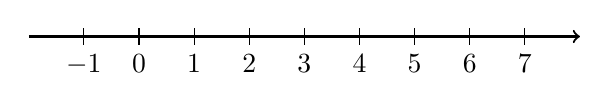
\begin{tikzpicture}[scale=0.7]
  \draw[thick,->] (-2,0) -- (8,0);
  \foreach \x in {-1,...,7} \draw (\x,0.15) -- (\x,-0.15) node[below] {$\x$};
\end{tikzpicture}
\end{center}
\end{questionText}
\correctAnswer{$x < 3$; open circle at $3$, shade left}
\explanation{Subtract $9$: $-3x > -9$. Divide by $-3$ and flip: $x < 3$. Open circle at $3$, shade left.}
\end{practiceQuestion}

\begin{practiceQuestion}{6-2-q30}{gsa}
\begin{questionText}
The grid below shows a house floor plan at scale $1$ square $= 3$ m. The shaded region represents the kitchen. If you redraw the plan at $1$ square $= 1$ m, how many grid squares will the new kitchen cover?

\begin{center}
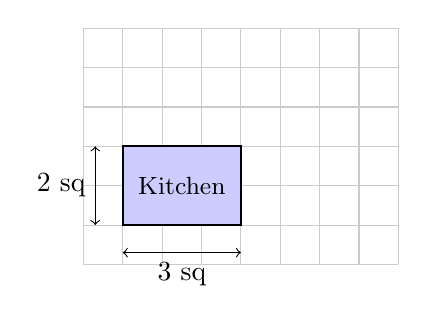
\begin{tikzpicture}[scale=0.5]
  \draw[step=1,gray!40,thin] (0,0) grid (8,6);
  \fill[blue!20] (1,1) rectangle (4,3);
  \draw[thick] (1,1) rectangle (4,3);
  \node at (2.5,2) {\small Kitchen};
  \draw[<->] (1,0.3) -- (4,0.3);
  \node[below] at (2.5,0.3) {$3$ sq};
  \draw[<->] (0.3,1) -- (0.3,3);
  \node[left] at (0.3,2) {$2$ sq};
\end{tikzpicture}
\end{center}
\end{questionText}
\correctAnswer{$54$ grid squares}
\explanation{Original kitchen: $3$ squares by $2$ squares $= 6$ squares. Each original square represents $3$ m, new square represents $1$ m. Scale ratio for length: $\frac{3}{1} = 3$. New dimensions: $3 \times 3 = 9$ squares by $2 \times 3 = 6$ squares. New area: $9 \times 6 = 54$ grid squares.}
\end{practiceQuestion}

\begin{practiceQuestion}{6-3-q24}{sa}
\begin{questionText}
You are given angles $45°$ and $45°$ and side $6$ cm between them. How many triangles can you draw?
\end{questionText}
\correctAnswer{Exactly one}
\explanation{ASA (two angles and the included side) fully determine a unique triangle. The third angle would be $180° - 45° - 45° = 90°$.}
\end{practiceQuestion}

\begin{practiceQuestion}{6-4-q19}{sa}
\begin{questionText}
Two angles of a triangle are $72°$ and $53°$. What is the third angle?
\end{questionText}
\correctAnswer{$55°$}
\explanation{$180° - 72° - 53° = 55°$.}
\end{practiceQuestion}

\begin{practiceQuestion}{6-5-q13}{mc}
\begin{questionText}
A hexagonal prism is sliced parallel to its base. What is the cross-section?
\end{questionText}
\choiceA{Rectangle}
\choiceB{Triangle}
\choiceC{Hexagon}
\choiceD{Circle}
\correctAnswer{C}
\explanation{Any cut parallel to the base of a prism gives a shape congruent to the base. A hexagonal prism has a hexagonal base, so the cross-section is a hexagon.}
\end{practiceQuestion}

\begin{practiceQuestion}{7-3-q16}{mc}
\begin{questionText}
A student says the area of a circle with radius $6$ cm is $37.68$ cm$^2$. What mistake did the student most likely make?
\end{questionText}
\choiceA{Used diameter instead of radius}
\choiceB{Calculated circumference instead of area}
\choiceC{Forgot to square the radius}
\choiceD{Divided by $2$ instead of squaring}
\correctAnswer{B}
\explanation{$C = 2\pi r = 2 \times 3.14 \times 6 = 37.68$. The student found circumference, not area. The area is $3.14 \times 36 = 113.04$ cm$^2$.}
\end{practiceQuestion}

\begin{practiceQuestion}{7-4-q09}{mc}
\begin{questionText}
A banner is shaped like a rectangle $18$ in by $6$ in with a triangle cut from one end. The triangle has a base of $6$ in and a height of $4$ in. What is the area of the banner?
\end{questionText}
\choiceA{$84$ in$^2$}
\choiceB{$96$ in$^2$}
\choiceC{$108$ in$^2$}
\choiceD{$120$ in$^2$}
\correctAnswer{B}
\explanation{Rectangle: $18 \times 6 = 108$ in$^2$. Triangle: $\frac{1}{2} \times 6 \times 4 = 12$ in$^2$. Banner: $108 - 12 = 96$ in$^2$.}
\end{practiceQuestion}

\begin{practiceQuestion}{7-5-q12}{mc}
\begin{questionText}
A storage box is in the shape of a cube with side $12$ inches. What is its surface area?
\end{questionText}
\choiceA{$144$ in$^2$}
\choiceB{$432$ in$^2$}
\choiceC{$864$ in$^2$}
\choiceD{$1728$ in$^2$}
\correctAnswer{C}
\explanation{$SA = 6s^2 = 6 \times 144 = 864$ in$^2$.}
\end{practiceQuestion}

\begin{practiceQuestion}{7-6-q08}{mc}
\begin{questionText}
A storage container is $2$ ft long, $1.5$ ft wide, and $3$ ft tall. How many cubic feet can it hold?
\end{questionText}
\choiceA{$6$ ft$^3$}
\choiceB{$6.5$ ft$^3$}
\choiceC{$9$ ft$^3$}
\choiceD{$10$ ft$^3$}
\correctAnswer{C}
\explanation{$V = 2 \times 1.5 \times 3 = 9$ ft$^3$.}
\end{practiceQuestion}

\begin{practiceQuestion}{8-1-q26}{gmc}
\begin{questionText}
A student surveyed $50$ classmates about their favorite fruit. The results are shown in the bar graph below.

\begin{center}
\begin{tikzpicture}[scale=0.7]
  \draw[thick,->] (0,0) -- (0,6.5) node[above]{\small Number of Students};
  \draw[thick,->] (0,0) -- (8.5,0);
  % bars
  \fill[funBlue!70] (0.5,0) rectangle (1.5,4);
  \fill[funGreen!70] (2.5,0) rectangle (3.5,3);
  \fill[funOrange!70] (4.5,0) rectangle (5.5,2);
  \fill[funRed!70] (6.5,0) rectangle (7.5,1);
  % labels
  \node[below] at (1,0) {\small Apple};
  \node[below] at (3,0) {\small Banana};
  \node[below] at (5,0) {\small Orange};
  \node[below] at (7,0) {\small Grape};
  % y-axis ticks
  \foreach \y in {1,2,3,4,5,6} {
    \draw (-0.1,\y) -- (0.1,\y);
    \node[left] at (0,\y) {\small $\y\times5$};
  }
  % values on bars
  \node[above] at (1,4) {\small $20$};
  \node[above] at (3,3) {\small $15$};
  \node[above] at (5,2) {\small $10$};
  \node[above] at (7,1) {\small $5$};
\end{tikzpicture}
\end{center}

If there are $500$ students in the school, predict how many prefer apples.
\end{questionText}
\choiceA{$20$}
\choiceB{$100$}
\choiceC{$200$}
\choiceD{$250$}
\correctAnswer{C}
\explanation{$\frac{20}{50} = 40\%$ prefer apples. $40\%$ of $500 = 200$.}
\end{practiceQuestion}

\begin{practiceQuestion}{8-3-q13}{mc}
\begin{questionText}
The difference between the means of two groups is $10$. The MAD for each group is $2$. How many MADs apart are the means?
\end{questionText}
\choiceA{$2$}
\choiceB{$5$}
\choiceC{$10$}
\choiceD{$20$}
\correctAnswer{B}
\explanation{$\frac{10}{2} = 5$ MADs apart.}
\end{practiceQuestion}

\begin{practiceQuestion}{8-4-q15}{mc}
\begin{questionText}
Why is it important to use multiple measures (mean, median, range, IQR, MAD) when comparing two groups?
\end{questionText}
\choiceA{One measure tells the complete story}
\choiceB{Using more measures wastes time}
\choiceC{Different measures reveal different aspects of the data}
\choiceD{All measures always give the same conclusion}
\correctAnswer{C}
\explanation{Mean and median show center; range, IQR, and MAD show spread. Together they give a complete picture.}
\end{practiceQuestion}

\begin{practiceQuestion}{8-7-q19}{sa}
\begin{questionText}
A frequency table shows: Soccer $15$, Basketball $20$, Tennis $10$, Swimming $5$. What is the total and what percent play basketball?
\end{questionText}
\correctAnswer{Total $= 50$; Basketball $= 40\%$}
\explanation{$15+20+10+5 = 50$. Basketball: $\frac{20}{50} = 40\%$.}
\end{practiceQuestion}

\begin{practiceQuestion}{9-4-q30}{gsa}
\begin{questionText}
The table below shows a probability model for a game spinner. One probability is missing. Find the missing probability for outcome D.

\begin{center}
\begin{tabular}{|c|c|}
\hline
\textbf{Outcome} & \textbf{Probability} \\
\hline
A & $0.30$ \\
\hline
B & $0.25$ \\
\hline
C & $0.15$ \\
\hline
D & ? \\
\hline
\end{tabular}
\end{center}
\end{questionText}
\correctAnswer{$0.30$}
\explanation{$P(D) = 1 - (0.30 + 0.25 + 0.15) = 1 - 0.70 = 0.30$.}
\end{practiceQuestion}

\begin{practiceQuestion}{9-6-q06}{mc}
\begin{questionText}
Two dice are rolled. What is the probability that both dice show the same number (doubles)?
\end{questionText}
\choiceA{$\frac{1}{36}$}
\choiceB{$\frac{1}{12}$}
\choiceC{$\frac{1}{6}$}
\choiceD{$\frac{1}{3}$}
\correctAnswer{C}
\explanation{Doubles: $(1,1), (2,2), (3,3), (4,4), (5,5), (6,6)$ — that is $6$ out of $36$. $P = \frac{6}{36} = \frac{1}{6}$.}
\end{practiceQuestion}

\begin{practiceQuestion}{9-7-q25}{sa}
\begin{questionText}
A student runs $200$ simulation trials for an event with theoretical probability $\frac{1}{4}$. They observe the event $54$ times. What is the experimental probability? Is it close to the theoretical value?
\end{questionText}
\correctAnswer{$0.27$; yes, it is close to $0.25$}
\explanation{$P = \frac{54}{200} = 0.27$. Theoretical $= 0.25$. The difference of $0.02$ is small, especially with $200$ trials.}
\end{practiceQuestion}
